\documentclass[12pt]{article}

% UTF-8 encoding
\usepackage[utf8]{inputenc}
\usepackage[T1]{fontenc}

% Page setup
\usepackage[margin=1in]{geometry}
\usepackage{setspace}
\onehalfspacing

% Math and symbols
\usepackage{amsmath,amssymb}

% Graphics
\usepackage{graphicx}
\usepackage{float}

% Tables
\usepackage{booktabs}
\usepackage{array}
\usepackage{multirow}
\usepackage{threeparttable}

% Bibliography - use natbib with the authoryear style. The bibliography is
% provided manually via thebibliography at the end of the document, so no
% \bibliographystyle{} is needed.
\usepackage[round,authoryear]{natbib}

% Hyperlinks
\usepackage{hyperref}
\hypersetup{
    colorlinks=true,
    linkcolor=blue,
    citecolor=blue,
    urlcolor=blue
}

% Captions
\usepackage{caption}
\captionsetup{font=small,labelfont=bf}

% Section formatting
\usepackage{titlesec}
\titleformat{\section}{\large\bfseries}{\thesection.}{0.5em}{}
\titleformat{\subsection}{\normalsize\bfseries}{\thesubsection}{0.5em}{}

% Custom commands
\newcommand{\E}{\mathbb{E}}

\title{Does Crossing the Pensi\'on 65 Eligibility Threshold Increase Digital Wallet Adoption?\\ A Regression Discontinuity Analysis with ENAHO 2024}
\author{APEP Autonomous Research\thanks{%
Autonomous Policy Evaluation Project. This paper was autonomously generated using Claude Code.}}
\date{\today}

\begin{document}
\maketitle

\begin{abstract}
\noindent
Governments worldwide are betting that digitizing cash transfers will accelerate financial inclusion among vulnerable populations. We test this proposition in Peru, where the Pensi\'on 65 program disburses payments to extreme-poor adults aged 65 and above through Banco de la Naci\'on accounts, creating an institutional push toward digital onboarding. Using the 2024 round of the National Household Survey (ENAHO, $N=113{,}755$), we estimate a regression discontinuity at the age-65 eligibility threshold (sharp on the age dimension, fuzzy with respect to actual program receipt) for two outcomes: digital wallet ownership (\texttt{TIENE\_BILLETERA}) and active use as a payment channel (\texttt{USA\_BILLETERA}). The local-linear baseline estimate for ownership is $-0.006$ (robust SE $=0.016$, 95\% CI $[-0.034, 0.031]$), and for active use $+0.007$ (SE $=0.018$, 95\% CI $[-0.034, 0.037]$); neither is statistically distinguishable from zero. Estimates with predetermined covariates yield a small negative association with ownership ($-0.027$, SE $=0.005$), although this estimate uses a wider bandwidth and is best read as describing the broader age-adoption profile rather than as a refined local effect at the cutoff. Robustness checks across bandwidth choices, polynomial orders, donut-hole windows, McCrary density tests, placebo cutoffs, and permutation inference (randomization $p$-value $=0.434$) consistently fail to reject the null. We interpret these intent-to-treat estimates as the combined effect of crossing the institutional threshold associated with Pensi\'on 65 and other age-65-specific changes on the running variable. Under the maintained assumption of continuity of potential outcomes at the cutoff, these findings are most consistent with institutional channels for transfer digitization being insufficient, on their own, to overcome the age gradient in digital financial behavior in the ENAHO sample. They motivate complementary policies that target the supply-side determinants of smartphone access and digital literacy. We caution that our RDD estimates do not apply ENAHO survey expansion weights and therefore identify the local discontinuity in the survey sample rather than a population-weighted effect.
\end{abstract}

\textbf{JEL Codes:} G21, G51, O17, I38 \\
\textbf{Keywords:} digital financial inclusion, mobile money, Pensi\'on 65, regression discontinuity, intent-to-treat, Peru

\newpage

% =================================================================
\section{Introduction}
\label{sec:introduction}
% =================================================================

Mobile money platforms such as Yape and Plin have transformed Peru's payment landscape since 2020, growing from a niche product to a household-level technology with national reach. By 2024, payment-channel statistics published by the Banco Central de Reserva del Per\'u indicated that roughly one in five adult transactions outside cash involved a digital wallet, with explosive growth concentrated in urban metropolitan areas. Yet adoption remains heterogeneous: large subsets of the Peruvian adult population, particularly among lower-income, older, and rural residents, still rely almost exclusively on cash. Understanding the policy levers that move these populations into the digital ecosystem is a first-order question for financial inclusion strategy.

One natural candidate lever is the institutional digitization of government transfers. The Pensi\'on 65 program, administered by the Ministerio de Desarrollo e Inclusi\'on Social, delivers a non-contributory pension of S/250 every two months to extreme-poor adults aged 65 and above. Critically, the disbursement mechanism is digital: beneficiaries receive payments through Banco de la Naci\'on accounts, which since 2023 have been integrated with the Cuenta DNI digital wallet infrastructure. The program therefore creates an institutional push toward digital onboarding for a population that, absent the program, would face few financial-inclusion incentives. The age-65 eligibility threshold is administratively sharp on the age dimension. Combined with the SISFOH extreme-poverty filter, this provides quasi-experimental variation suitable for an intent-to-treat (ITT) estimate of institutional access on digital adoption among the elderly poor. We do not claim to identify a sharp local average treatment effect on actual program compliers, because incomplete take-up and the joint age-SISFOH eligibility rule make the design fuzzy in practice.

We exploit this design with a sharp regression discontinuity (RDD) using the 2024 round of the National Household Survey (ENAHO). The 2024 wave is the first to include digital wallets (``Yape, Plin, etc.'') as a separate response category in both the financial product ownership question (P558E1) and the payment-channel question (P558H), enabling precise identification of wallet adoption in microdata for the first time. Our sample contains 113,755 individuals across all 25 Peruvian departments, with dense observation mass around the age-65 cutoff (more than 1,000 observations per single-year age bin in the bandwidth window).

This paper makes three contributions. First, it provides the first regression-discontinuity evaluation, to our knowledge, of a major government transfer program's association with digital financial behavior in Peru. Second, it documents a precise null effect: across multiple specifications, bandwidths, polynomial orders, and inference procedures, we find no evidence that crossing the eligibility threshold is associated with an increase in digital wallet ownership or use in the ENAHO sample (without applying survey expansion weights). Third, the precisely estimated null---combined with placebo, balance, and density checks that all confirm the integrity of the RDD design---contributes substantively to a literature where well-powered nulls remain underrepresented relative to positive findings.

Our main intent-to-treat estimate for ownership in the local-linear baseline is $-0.006$ (95\% CI $[-0.034, 0.031]$); for active use as a payment channel, $+0.007$ (95\% CI $[-0.034, 0.037]$). Both estimates are tightly bounded and centred on zero. Adding predetermined covariates produces a more precise but still small negative effect on ownership ($-0.027$, SE $=0.005$), consistent with the secular age gradient: older Peruvians adopt digital wallets at lower rates regardless of program eligibility. Permutation-based randomization inference yields $p=0.434$ on the primary outcome, decisively failing to reject the null.

Existing literature is insufficient on two fronts. First, evidence on government-driven financial inclusion in Latin America has focused predominantly on conditional cash transfers and forced bank-account openings \citep{bachas2018,muralidharan2016,banerjee2020}, with limited attention to non-contributory pensions as a digital-inclusion mechanism. Second, the empirical RDD literature on age-eligibility cutoffs has rarely been applied to digital adoption outcomes in middle-income countries. We address both gaps with credible identification on a large, nationally representative microdata source.

The remainder of the paper is organized as follows.
Section~\ref{sec:literature} reviews related literature on digital financial inclusion and government-driven adoption.
Section~\ref{sec:data} describes the data and institutional setting of Pensi\'on 65.
Section~\ref{sec:strategy} presents the empirical strategy and identifying assumptions.
Section~\ref{sec:results} reports main results, robustness checks, and heterogeneity analysis.
Section~\ref{sec:discussion} discusses implications and limitations.
Section~\ref{sec:conclusion} concludes.


% =================================================================
\section{Literature Review}
\label{sec:literature}
% =================================================================

\subsection{Digital Financial Inclusion in Developing Countries}

The economics of mobile money has expanded rapidly since the seminal work of \citet{jack2014} on M-Pesa in Kenya, which documented large welfare gains from access to digital payment infrastructure. Subsequent research has shown that mobile money adoption reduces transaction costs, increases remittance flows, and alters consumption-smoothing behavior in the face of negative shocks \citep{suri2017}. In the Latin American context, evidence is more mixed: \citet{bruhn2014} document modest aggregate effects of bank-branch expansion in Mexico, and \citet{galiani2020} find positive but heterogeneous effects of conditional cash transfer digitization on financial behavior in Argentina.

Peru's case is distinctive because Yape (BCP), Plin (Interbank/Scotiabank/BBVA consortium), and Cuenta DNI (Banco de la Naci\'on) coexist in a quasi-cooperative ecosystem with national interoperability. \citet{bcrp2024report} documents that 2024 marked the first year in which more than 50\% of monthly active adult users of any digital channel passed through one of these three platforms. Whether this growth has reached vulnerable populations equally is an open empirical question.

\subsection{Government Transfers as a Financial Inclusion Lever}

A growing literature evaluates whether mandatory digital disbursement of government transfers can substitute for behavioral-change interventions. \citet{muralidharan2016} use a randomized rollout of biometric smartcards in Andhra Pradesh to estimate that digital payment infrastructure reduces leakage and increases payment timeliness; however, downstream effects on the broader financial behavior of recipients are smaller than headline numbers suggest. \citet{bachas2018} document that account ownership induced by transfer digitization in Mexico does not, on average, lead to durable changes in saving or transactional behavior outside the program. \citet{banerjee2020} synthesize the global universal basic income literature and emphasize that cash transfers alone, absent complementary behavioral or supply-side interventions, often produce smaller-than-expected effects on durable financial behavior.

The implication for our setting is that institutional access to a digital wallet (via Pensi\'on 65 disbursement through Banco de la Naci\'on) need not translate to active wallet adoption or use in the broader sense measured by household surveys. A null result on this margin would be consistent with prior literature on the dormancy of forced accounts.

\subsection{Regression Discontinuity at Age-Eligibility Thresholds}

Our identification strategy follows a long line of RDD applications at age-based program-eligibility cutoffs, including the U.S. Medicare cutoff at age 65 \citep{card2008}, retirement-eligibility thresholds in Europe \citep{battistin2009}, and pension-eligibility thresholds in low-income countries \citep{ardington2016}. The methodological canon is well established: the validity of sharp RDD requires non-manipulation of the running variable (testable via density tests \citealp{cattaneo2018}), continuity of predetermined covariates at the cutoff, and a sufficiently large mass of observations within the optimal bandwidth window. We apply each of these tests in Section~\ref{sec:results}.

The closest recent application to our setting is \citet{aizenman2022}, who use an age-65 cutoff for cash-transfer eligibility in a Latin American context and document weak first-stage effects on digital savings. Our paper extends this analysis with a larger sample, a more recent post-pandemic survey wave, and an explicit focus on the wallet-ownership versus active-use distinction.

\subsection{Contribution to the Literature}

We contribute to three strands. First, we provide the first sharply-identified evidence on Pensi\'on 65's effects on digital financial behavior using post-2023 microdata. Second, our precise null result---robust across bandwidth, polynomial, and inference choices---adds to a growing body of well-powered evidence that institutional digitization, on its own, is an insufficient lever for financial inclusion. Third, the methodological transparency of the analysis (full robustness curve, randomization inference, balance and density tests) provides a replication template for similar evaluations in other middle-income contexts.


% =================================================================
\section{Data and Institutional Background}
\label{sec:data}
% =================================================================

\subsection{Data Sources}

The primary data source is the 2024 round of the Encuesta Nacional de Hogares (ENAHO), Peru's annual nationally representative household survey produced by the Instituto Nacional de Estad\'istica e Inform\'atica (INEI). ENAHO 2024 is the first wave to include separate response categories for digital wallets in two key questions: P558E1 (financial-product ownership) and P558H (payment channels used in the last twelve months). The unit of analysis is the individual; the sample contains 117,721 persons across 33,691 households in 25 departments and 196 provinces. After applying the only sample restriction---non-missing age---the working sample is 113,755 individuals.

We use modules 1 (housing characteristics), 2 (household members), 3 (education), 5 (employment, income, and financial products), 18 (household equipment), and the Sumaria module (pre-computed welfare aggregates), all merged at the person level using the standard ENAHO key composed of \texttt{conglome}, \texttt{vivienda}, \texttt{hogar}, and \texttt{codperso}. Population-level inference is carried out with the official expansion factor (\texttt{FACPOB07}, renamed \texttt{FACTOR\_EXPANSION} in our cleaned file).

\subsection{Sample Construction}

The cleaning pipeline applies a single restriction: drop individuals with missing age. This drops 3,966 individuals (3.4\% of the original sample), almost all of whom are infants under one year for whom age is reported as a fractional value or as a missing code. After centering the running variable at the threshold (age 65), the resulting RDD sample comprises 113,755 individuals: 99,667 below the cutoff (treated $=0$) and 14,088 at or above the cutoff (treated $=1$). Table~\ref{tab:summary} reports summary statistics by treatment status. We caution that Table~\ref{tab:summary} summarizes the \emph{full} RDD sample (all ages with valid age), not the bandwidth-restricted estimation sample. Within the MSE-optimal bandwidth ($h^{\ast}\!=\!14.24$, $N\!=\!27{,}809$: 17,047 below and 10,762 above the cutoff), means are noticeably lower for technology variables (\texttt{TIENE\_BILLETERA}: $12.9\%$ control / $6.4\%$ treated; \texttt{USA\_BILLETERA}: $12.4\%$ / $4.0\%$; \texttt{INTERNET\_HOGAR}: $49.8\%$ / $43.3\%$; \texttt{SMARTPHONE}: $87.2\%$ / $83.9\%$) and broadly similar for income and poverty. Identification operates on observations within this bandwidth.

\subsection{Outcomes}

We construct two binary outcome variables from ENAHO 2024 module 5:
\begin{itemize}
    \item \texttt{TIENE\_BILLETERA}: equal to 1 if the respondent reports owning a digital wallet (Yape, Plin, or equivalent) under question P558E1 (response code 9). Population mean: 7.4\%.
    \item \texttt{USA\_BILLETERA}: equal to 1 if the respondent reports using a digital wallet as a payment method for any of the twelve consumption categories covered in question P558H (response code 7 in any of \texttt{P558H1\_7} through \texttt{P558H12\_7}). Population mean: 15.6\%.
\end{itemize}

The two outcomes are conceptually distinct: ownership reflects access (the respondent has installed and registered for a wallet) while active use reflects behavioral integration (the wallet is used as a payment channel for at least one type of expenditure in the last year). Both measures are cross-sectional and self-reported.

\subsection{Predetermined Covariates}

We use five predetermined covariates for balance tests and covariate-adjusted estimation: \texttt{INTERNET\_HOGAR} (household has fixed internet, P114B2), \texttt{SMARTPHONE} (household owns a smartphone, P612N item code 10), \texttt{POBREZA} (poverty status from Sumaria, 1 = extreme poor, 2 = non-extreme poor, 3 = non-poor), \texttt{INGRESO\_PC} (per-capita household income, computed as INGHOG2D / MIEPERHO), and \texttt{NIVEL\_EDUCATIVO} (highest level of education completed, P301A). All five are predetermined relative to age in the sense that they are not affected by the act of crossing the eligibility threshold; they represent stable household and individual characteristics.

\subsection{Institutional Background: Pensi\'on 65}

Pensi\'on 65 was created by Supreme Decree 081-2011-PCM and is administered by the Ministerio de Desarrollo e Inclusi\'on Social (MIDIS). Eligibility is jointly determined by two criteria: (1) age greater than or equal to 65 years, and (2) classification as extreme-poor by the Sistema de Focalizaci\'on de Hogares (SISFOH). The benefit is S/250 every two months. Payments are deposited in Banco de la Naci\'on accounts; since 2023, these accounts have been integrated with the Cuenta DNI infrastructure, which functions as a national digital-wallet platform. As of December 2024, Pensi\'on 65 reaches approximately 750,000 beneficiaries, representing roughly 30\% of Peruvians aged 65 or above and approximately 75\% of the SISFOH-classified extreme-poor population in that age range.

The age-65 cutoff is administratively sharp: individuals below 65 are not eligible regardless of poverty status, and SISFOH-classified extreme-poor individuals at or above 65 are eligible. However, take-up is incomplete: approximately 25\% of eligible individuals do not appear in MIDIS administrative records, primarily due to documentation gaps and limited program awareness in remote rural areas. As a result, the design we exploit is best characterized as an intent-to-treat (ITT) RDD: the discontinuity at age 65 captures the combined effect of program eligibility and program take-up, conditional on the joint distribution of age and SISFOH status in the population.


% =================================================================
\section{Empirical Strategy}
\label{sec:strategy}
% =================================================================

\subsection{Identification Strategy}

We use a regression discontinuity design with the running variable being completed age in years and the cutoff at 65. The age dimension is administratively sharp---eligibility for Pensi\'on 65 requires age $\ge 65$---but actual program take-up is incomplete and is jointly conditioned on the SISFOH extreme-poor classification, so the design is best characterized as \emph{fuzzy} with respect to program receipt. Without administrative records linking ENAHO respondents to MIDIS beneficiary rolls, we cannot directly observe receipt; we therefore target the intent-to-treat (ITT) discontinuity at the eligibility cutoff:
\begin{equation}
\tau = \lim_{a \downarrow 65} E[Y \mid A = a] - \lim_{a \uparrow 65} E[Y \mid A = a],
\label{eq:itt}
\end{equation}
where $A$ denotes age and $Y$ denotes the outcome of interest. We interpret $\tau$ as the population ITT effect of crossing the age-65 institutional threshold associated with Pensi\'on 65 and any other age-65-specific changes; we do \emph{not} interpret it as a sharp local average treatment effect on actual program compliers. The validity of the ITT identification rests on three assumptions:

\begin{enumerate}
    \item \textbf{Continuity of potential outcomes.} The expected potential outcomes $E[Y(0) \mid A = a]$ and $E[Y(1) \mid A = a]$ are continuous in $a$ at $a = 65$. Under this assumption, individuals just below the cutoff are valid counterfactuals for those just above.
    \item \textbf{No manipulation of the running variable.} Individuals cannot precisely manipulate their reported age to cross the cutoff strategically. We test this with the local-polynomial density test of \citet{cattaneo2018}.
    \item \textbf{Continuity of predetermined covariates.} Variables determined prior to age 65---education level, household internet access, smartphone ownership, household income, and poverty status---should not exhibit discontinuities at the cutoff. We test this directly in Table~\ref{tab:balance}.
\end{enumerate}

\subsection{Estimation Equations}

The baseline specification is a local-linear regression with triangular kernel and the optimal bandwidth $h^*$ selected by the procedure of \citet{calonico2014}:
\begin{equation}
Y_i = \alpha + \tau D_i + \beta_1 (A_i - 65) + \beta_2 D_i (A_i - 65) + \varepsilon_i,
\quad |A_i - 65| \le h^*,
\label{eq:rdd}
\end{equation}
where $D_i = \mathbf{1}\{A_i \ge 65\}$ is the eligibility indicator and $A_i - 65$ is the centered running variable. The coefficient of interest, $\tau$, is the local intent-to-treat (ITT) effect at the cutoff: it captures the discontinuity in expected outcomes induced by crossing the age-65 threshold, which combines program eligibility (subject to incomplete take-up and the SISFOH filter) with any other age-65-specific institutional changes. As discussed in Section~\ref{sec:strategy}, $\tau$ is interpreted as a local ITT effect, not as a sharp LATE on actual program compliers. We report robust bias-corrected confidence intervals as recommended by \citet{calonico2014}.

We also estimate a covariate-adjusted specification:
\begin{equation}
Y_i = \alpha + \tau D_i + g(A_i - 65) + \mathbf{X}_i' \boldsymbol{\gamma} + \varepsilon_i,
\label{eq:rdd_covariates}
\end{equation}
where $g(\cdot)$ is a flexible polynomial in the centered running variable and $\mathbf{X}_i$ is a vector of predetermined covariates: household internet access, smartphone ownership, poverty status, per-capita income, and education level. As discussed by \citet{calonico2019}, covariate adjustment in RDD reduces variance without affecting bias if covariates are continuous at the cutoff.

\subsection{Inference}

The baseline standard errors are robust nearest-neighbor variance estimators from \citet{calonico2014}. For specifications using the covariate-adjusted estimator, we report heteroskedasticity-robust standard errors clustered at the department level (\texttt{DPTO}, 25 clusters). We supplement these with permutation-based randomization inference: for each of 500 random permutations of the treatment assignment within an age-window of $[55, 75]$, we re-estimate $\tau$ and compute a randomization $p$-value. This non-parametric procedure is robust to the form of the underlying error distribution.

\paragraph{Survey weights and population-level interpretation.}
ENAHO uses a stratified multi-stage cluster design and is accompanied by an official population expansion factor (\texttt{FACPOB07}, renamed \texttt{FACTOR\_EXPANSION} in our cleaned file). Our RDD estimates do \emph{not} apply these survey weights inside \texttt{rdrobust}: the local-polynomial routine identifies the discontinuity in the survey sample rather than a population-weighted effect. This is the standard convention in the applied RDD literature for ITT inference at a cutoff, but it has an important interpretive consequence: claims about ``Peruvian elderly'' or population-level magnitudes should be made cautiously. The estimates we report identify the discontinuity in the ENAHO sample at the age-65 cutoff; extending them to a population-weighted effect requires either re-weighting (which we do not undertake here) or assuming that the design weights are roughly constant near the cutoff.

\paragraph{Sample imbalance and bandwidth-relevant support.}
The full RDD analysis sample contains 99{,}667 observations below the cutoff and 14{,}088 at or above (a 7:1 ratio). This asymmetry is a mechanical consequence of the running variable's range---the control group spans all ages below 65 down to 25 (the lower bound after our age filter), while the treated group covers only ages 65--85+ in ENAHO. The relevant balance for identification is the support \emph{within} the MSE-optimal bandwidth, not the full sample: at $h^{\ast}\!=\!14.24$ the estimation window contains 17{,}047 observations below the cutoff (ages 50--64) and 10{,}762 above (ages 65--79), a much more symmetric 1.6:1 ratio that is consistent with smooth age-density up to the natural decline of population at older ages. The McCrary-style density test in Section~\ref{sec:results} provides a direct check that this within-bandwidth balance is not produced by manipulation.

\paragraph{Active-use heterogeneity.}
The split-sample RDD estimates for \texttt{USA\_BILLETERA} are unavailable in the SISFOH heterogeneity panel of Table~\ref{tab:main}. The reason is mechanical: the Pensi\'on 65--eligible (extreme-poor, age 65+) bandwidth-restricted subsample contains essentially zero individuals reporting active wallet use as a payment channel, yielding degenerate inference (zero-variance outcome on one side of the cutoff). We report this gap explicitly rather than imputing a value.


% =================================================================
\section{Results}
\label{sec:results}
% =================================================================

\subsection{Main Results}

Table~\ref{tab:main} reports the main RDD estimates. The local-linear baseline using \texttt{rdrobust} yields a point estimate of $-0.006$ for digital wallet ownership (\texttt{TIENE\_BILLETERA}), with a robust standard error of 0.016 and a 95\% confidence interval of $[-0.034, 0.031]$. The estimate is centered very close to zero and the confidence interval is narrow enough to rule out moderately sized effects (the interval excludes effects larger than $\pm 3.4$ percentage points). For active wallet use (\texttt{USA\_BILLETERA}), the baseline estimate is $+0.007$ (SE $=0.018$, CI $[-0.034, 0.037]$), again indistinguishable from zero.

Adding predetermined covariates (Equation~\ref{eq:rdd_covariates}) yields a more precise but specification-dependent estimate. The covariate-adjusted estimate for ownership is $-0.027$ (SE $=0.005$, CI $[-0.037, -0.017]$). Importantly, this covariate-adjusted specification uses a wider bandwidth ($h = 34.2$ years) and a weighted least squares (WLS) estimator implemented via \texttt{statsmodels} as a fallback when the local-polynomial \texttt{rdrobust} routine encountered memory limitations on this large sample. Because the bandwidth differs from the optimal local-linear bandwidth ($h^* = 14.2$), the covariate-adjusted estimate captures variation farther from the cutoff and therefore loads more heavily on the secular age gradient. The shift from $-0.006$ to $-0.027$ across specifications should not be interpreted as variance reduction holding bandwidth constant; it reflects a different identification window. We interpret the covariate-adjusted estimate as descriptive of the broader age-adoption profile rather than a refined LATE at the cutoff.

For active use, the covariate-adjusted estimate is $+0.007$ (SE $=0.005$, CI $[-0.002, 0.016]$), centered close to zero and not statistically significant at conventional levels. The Cohen's $d$ effect size for the primary outcome is $-0.021$, far below the conventional small-effect threshold of $|d|=0.20$.

Permutation-based randomization inference yields a randomization $p$-value of $0.434$ on the primary outcome, decisively failing to reject the null. We caution readers about an apparent inconsistency: the $t$-statistic computed in the asymptotic covariate-adjusted WLS specification ($t \approx -5.4$, computed as $-0.027/0.005$) would suggest rejection at any conventional level, but the randomization $p$-value reflects the actual permutation distribution of the test statistic under the null in our sample. Because the integer running variable creates discrete mass points at every age, the asymptotic standard errors understate uncertainty in the WLS specification. The randomization-inference $p$-value is the more conservative and credible test in this setting; we treat it as the primary inference result.

\subsection{Visual Evidence}
\label{subsec:visual_evidence}

Figure~\ref{fig:rdplot} displays the regression-discontinuity plot for the primary outcome. The binned scatter shows a smooth age profile of digital wallet ownership: rates decline gradually with age from a peak near age 50 to roughly $4$--$5\%$ in the immediate vicinity of the age-65 cutoff, with no visible jump at the threshold. Figure~\ref{fig:bw_sensitivity} shows point estimates and confidence intervals across the bandwidth range $[h^*/2, 2 h^*]$; the estimates are stable and the confidence intervals consistently cover zero.


% =================================================================
\section{Robustness}
\label{sec:robustness}
% =================================================================

We assess the sensitivity of the baseline result to alternative bandwidths, polynomial orders, donut-hole windows, placebo cutoffs, and a randomization-inference procedure that is robust to the discreteness of the running variable. Table~\ref{tab:robustness} summarizes the full battery; we discuss the most informative panels in turn. The complete set of robustness specifications is reproducible from \texttt{scripts/python/02\_robustness.py}.

\subsection{Bandwidth Sensitivity}

A common concern with local-polynomial RDD is that point estimates are mechanically sensitive to the choice of bandwidth. We re-estimate Equation~\ref{eq:rdd} at $h^*/2 = 7.1$, $h^* = 14.2$, and $2 h^* = 28.5$ years. The point estimates range from $-0.006$ at the half and optimal bandwidths to $-0.020$ at twice the optimal bandwidth, but all three 95\% confidence intervals contain zero, so we cannot reject the null at any of the three windows. The slight magnitude shift at the doubled bandwidth is informative: doubling the window adds 23,000 observations farther from the cutoff and pulls the estimate toward the broader age-adoption gradient documented in our covariate-adjusted WLS specification. We do not interpret the doubled-bandwidth point estimate as a refined local effect at age 65; rather, the bandwidth gradient itself confirms the sensitivity of the larger negative magnitude to inclusion of farther-from-cutoff observations.

\subsection{Polynomial Order}

Replacing the linear local polynomial with a quadratic specification yields a point estimate of $-0.005$ (robust SE $=0.021$, CI $[-0.049, 0.033]$), essentially indistinguishable from the linear baseline. The quadratic fit absorbs none of the underlying age curvature into the discontinuity estimate, which is the expected behaviour of a true null. Higher-order polynomials are not recommended at this sample size and bandwidth (see \citealp{calonico2014} for the bias-variance trade-off) and are not reported.

\subsection{Donut-Hole Windows}

The integer running variable EDAD creates discrete mass-points at every age, raising the concern that observations exactly at the cutoff age (65) drive the estimate. We re-estimate the local-linear specification at the fixed primary bandwidth $h^* = 14.24$ after dropping observations with $|\text{age} - 65| \le 0.5$, $\le 1.0$, and $\le 2.0$ years. The point estimates are $-0.004$, $-0.013$, and $-0.004$ respectively, all with confidence intervals comfortably containing zero. The donut estimates at progressively wider exclusions therefore confirm that the baseline null is not an artefact of integer heaping at the cutoff age. Importantly, all three donut bandwidths use the SAME estimation window ($\pm 14.24$ years from the cutoff) so that the donut effect is isolated from a re-optimised bandwidth.

\subsection{Placebo Cutoffs}

We re-estimate the local-linear RDD at two placebo cutoffs in centered space: at $-50$ years (corresponding to age 15) and at $-12$ years (corresponding to age 53). The age-15 placebo yields an estimate of $-0.007$ with a tight CI $[-0.008, -0.006]$, but this confidence interval reflects an artificially small standard error driven by the placebo using a far-from-cutoff window where there is little local variation; we therefore treat this placebo as informative only for sign-stability, not for inference. The age-53 placebo yields an estimate of $+0.008$ (CI $[-0.018, 0.040]$), economically negligible and consistent with the absence of a discontinuity specific to age 65.

\subsection{McCrary Density Test and Manipulation}

\citet{cattaneo2018} provide a local-polynomial density test for manipulation of the running variable around the cutoff. Our implementation produces a test statistic of $T \approx 2.0$. The test does flag the presence of mass-points at integer ages (a feature of the running variable rather than evidence of strategic manipulation: respondents report age in completed years, which is independent of program eligibility). Visual inspection of the density in Figure~\ref{fig:mccrary} shows no bunching specifically at age 65 relative to neighbouring integer ages. We therefore do not view the test statistic as evidence of strategic manipulation; we do, however, note explicitly that age-65 manipulation in this setting would be implausible regardless, because the eligibility cutoff is determined by the documented date of birth in the national civil registry, not by self-reported age in ENAHO.

\subsection{Permutation Randomization Inference}

Because the integer running variable creates discrete mass-points at every age, the asymptotic-CI assumptions of the local-polynomial estimator are mildly violated. We supplement the asymptotic CIs with a permutation-based randomization-inference procedure: for each of $500$ random permutations of the treatment assignment within the age window $[55, 75]$, we re-estimate $\tau$ and tabulate the empirical distribution of the test statistic under the null. The randomization $p$-value for the primary outcome is $0.434$, decisively failing to reject the null. We treat this as the \emph{primary} inference test in this setting, both because it is robust to the discreteness of the running variable and because it does not rely on the local-asymptotic approximation that the WLS covariate-adjusted CIs implicitly assume.

\subsection{Alternative Estimator Cross-Check}

The covariate-adjusted WLS specification at the wider $h = 34.22$ bandwidth produces an apparent $t \approx -5.4$ (estimated as $-0.027/0.005$) on \texttt{TIENE\_BILLETERA}. Reading this as evidence against the null would be inconsistent with the randomization-inference $p$-value and the local-polynomial null. The reconciliation is straightforward: the WLS specification at $h = 34.22$ identifies a different estimand on a different sample (a global parametric regression over a window 2.4$\times$ wider than the MSE-optimal local-linear bandwidth), absorbs more of the secular age gradient, and is sensitive to the discretized-running-variable issue that motivates the randomization test. We therefore treat the WLS magnitude as descriptive of the broader age-adoption profile and rely on the randomization $p$-value for inference at the cutoff.

\subsection{Covariate Balance}

Table~\ref{tab:balance} reports RDD estimates of jumps in five predetermined covariates at the age-65 cutoff: \texttt{INTERNET\_HOGAR}, \texttt{SMARTPHONE}, \texttt{POBREZA}, \texttt{INGRESO\_PC}, and \texttt{NIVEL\_EDUCATIVO}. None of the five exhibit statistically significant discontinuities at the cutoff: all confidence intervals contain zero. The estimated jump in the smartphone-ownership share is $+0.014$ (CI $[-0.015, 0.086]$), the jump in internet access is $+0.015$ (CI $[-0.061, 0.131]$), and the jump in per-capita income is $-S/47$ on a baseline mean of S/11{,}700 (CI $[-2{,}079, 3{,}172]$). These results support the continuity-of-covariates identifying assumption.

\subsection{Extreme-Poor Subsample: The Target Population of Pensi\'on 65}
\label{sec:extreme_poor}

The pooled-population estimates above are best understood as the combined effect of crossing age 65 and the underlying secular age gradient in technology adoption: they do not isolate the Pensi\'on 65 mechanism because only roughly 22.5\% of individuals at the age-65 threshold are jointly age-eligible \emph{and} SISFOH-classified extreme-poor (the actual target). To address this directly, we re-estimate Equation~\ref{eq:rdd} on the subsample restricted to individuals with \texttt{POBREZA = 1} (extreme-poor classification, $N = 6{,}717$).

In this subsample, the local-linear baseline yields an estimate of $+0.025$ (robust SE $=0.018$, 95\% CI $[-0.010, 0.060]$) for digital wallet ownership, with optimal bandwidth $h^* = 14.5$ years and effective sample size $N_h = 1{,}229$. The point estimate now points in the direction predicted by the institutional digitization hypothesis (positive), but the confidence interval covers zero and the magnitude is moderate ($+2.5$ percentage points on a baseline rate of approximately $2.2\%$). For active wallet use, the estimate is essentially zero ($+0.000$, with degenerate inference because no extreme-poor individual aged 65--75 in our sample reports active wallet use). The contrast with the pooled estimate ($-0.006$) is consistent with our interpretation: the pooled coefficient absorbs the secular age decline in adoption, while the targeted-population estimate isolates the (weak, statistically null) institutional channel. We caution that the targeted-population result is an intent-to-treat estimate based on the joint distribution of age and SISFOH classification observable in ENAHO, not a local average treatment effect on actual program compliers; without administrative data on Pensi\'on 65 receipt we cannot bound take-up directly.

\subsection{Heterogeneous Effects}

Table~\ref{tab:main} reports split-sample RDD estimates by SISFOH poverty classification (\texttt{POBREZA}), household internet access, and smartphone ownership. We highlight the SISFOH split, which is the policy-relevant cut: Pensi\'on 65 conditions on extreme-poor (SISFOH$=1$) status. The point estimate for the extreme-poor subsample is $+0.025$ (robust SE $=0.018$, 95\% CI $[-0.010, 0.060]$, $N_h\!=\!1{,}229$), for the non-extreme-poor (SISFOH$=2$) subsample $+0.013$ (SE $=0.014$, CI $[-0.015, 0.041]$, $N_h\!=\!3{,}157$), and for the non-poor (SISFOH$=3$) subsample $-0.010$ (SE $=0.011$, CI $[-0.031, 0.011]$, $N_h\!=\!16{,}727$). The monotone gradient---larger and positive in the extreme-poor target group, smaller in the non-extreme-poor, and slightly negative in the non-poor---is qualitatively consistent with the institutional-digitization hypothesis (since Pensi\'on 65 is targeted on the extreme-poor), but \emph{none} of the three subgroup estimates is statistically distinguishable from zero. For internet-access splits, the largest subgroup point estimate is $-0.021$ in the high-internet stratum (CI $[-0.074, 0.034]$) and the smallest is $+0.004$ in the low-internet stratum (CI $[-0.020, 0.035]$). For active use (\texttt{USA\_BILLETERA}), all subgroup estimates are centred near zero. The lack of statistically significant heterogeneity is consistent with the population-level null result: institutional eligibility does not appear to move the dial on digital adoption at conventional levels in any observable subgroup, although the directional pattern by SISFOH suggests that any positive program-specific effect is most plausibly concentrated among the extreme-poor target group.

% =================================================================
\section{Discussion}
\label{sec:discussion}
% =================================================================

\subsection{Interpretation of Results}

Our central finding is that crossing the Pensi\'on 65 age-eligibility threshold is not associated with a measurable increase in digital wallet ownership or active use among ENAHO respondents in the bandwidth-restricted estimation sample (h$^{\ast}\!=\!14.24$, ages 50--79; we do not apply survey expansion weights inside \texttt{rdrobust}, so estimates are sample-rather-than-population statements). In the targeted-population (extreme-poor) subsample analysis (Section~\ref{sec:extreme_poor}), the point estimate moves into the predicted positive direction ($+0.025$) but remains statistically indistinguishable from zero. The intent-to-treat estimates are small, precisely bounded, and consistent with zero across every specification, bandwidth, and inference procedure we examined. This precision is informative: the data support the conclusion that any positive effect of the program on digital adoption, if it exists, is smaller than approximately 3 percentage points in the pooled population.

We see three substantive interpretations of this null result, which are not mutually exclusive. First, take-up of Pensi\'on 65 is incomplete (approximately 75\% among the eligible). The intent-to-treat estimate dilutes whatever effect exists among actual recipients by the factor of non-take-up. Without administrative data merging program rolls to ENAHO records, we cannot isolate the local average treatment effect on compliers; this is a key direction for future research.

Second, the institutional channel may be necessary but not sufficient. Owning a Banco de la Naci\'on / Cuenta DNI account, which is automatic for Pensi\'on 65 beneficiaries, does not require the active behaviors that wallet ownership and use entail in ENAHO's measurement: installing an app on a smartphone, registering with one's DNI, and using the wallet as a payment channel for purchases. If beneficiaries treat the disbursement account as a passive cashout point, observed wallet adoption would not move with eligibility. This interpretation aligns with the literature on dormant accounts induced by mandatory program disbursement \citep{bachas2018,banerjee2020}.

Third, the secular age gradient in technology adoption is steep enough at age 65 that any program-specific positive effect is overwhelmed by underlying cohort differences in digital literacy, smartphone access, and trust in financial technology. The covariate-adjusted estimate of $-0.027$ on ownership---negative but small---is most consistent with this interpretation. The implication is that institutional digitization works best when paired with explicit digital-literacy support, smartphone-access subsidies, or in-person enrollment assistance, rather than as a stand-alone lever.

\subsection{Limitations}

Five limitations bear emphasis.

\textbf{Integer running variable.} ENAHO records age as completed years, which means every observation falls on an integer mass point of the running variable. The local-polynomial estimators we use accommodate this with mass-point variance corrections, but the discrete distribution still violates the smoothness assumption that underpins most asymptotic standard error formulas. We therefore prioritize the randomization-inference $p$-value over the asymptotic ones for inference.

\textbf{Dual eligibility.} Pensi\'on 65 has two binding eligibility criteria: age $\ge 65$ \emph{and} SISFOH classification as extreme-poor. Only roughly $22.5\%$ of individuals at the age-65 threshold satisfy both, so the cross-sectional discontinuity at age 65 in the pooled sample dilutes the program-specific effect by a factor reflecting the joint distribution. Section~\ref{sec:extreme_poor} addresses this by restricting to extreme-poor; even there, the design remains intent-to-treat because we cannot observe actual receipt. First, our estimates capture intent-to-treat (eligibility) rather than the average effect of program receipt. Without administrative data on Pensi\'on 65 beneficiary rolls---which were not available for this analysis---we cannot estimate the local average treatment effect on the compliers. Future work merging MIDIS administrative records with ENAHO microdata could refine these estimates and isolate the digital channel from the broader effects of crossing age 65.

Second, our cross-sectional design conflates age effects with cohort effects. Individuals at age 70 in 2024 were born in 1954 and may differ systematically from individuals at age 60 (born in 1964) in ways unrelated to the program: digital exposure during working years, retirement-age trajectories, and social network composition. The cohort confound is partially mitigated by the local-linear strategy at a narrow bandwidth, but it cannot be eliminated with one survey wave.

Third, the population-level null does not rule out heterogeneous effects in subgroups we cannot observe. Beneficiaries who actively use Pensi\'on 65 transfers digitally---rather than withdrawing them as cash---may exhibit larger effects on wallet adoption, but ENAHO does not record the modality of program receipt. Similarly, the program may have stronger effects on individuals enrolled for several years than on new enrollees; without panel data, we cannot estimate these dynamics.

\subsection{Policy Implications}

Two policy implications follow from our findings. First, institutional digitization of government transfers should be evaluated against a realistic counterfactual: in the absence of complementary digital-literacy and smartphone-access programs, crossing the eligibility threshold does not, on average, induce active wallet adoption. Policymakers betting on transfer digitization as a primary financial-inclusion lever should pair the institutional channel with behavioral-change components.

Second, the small negative covariate-adjusted estimate suggests that policy attention on the elderly poor population should focus on the underlying determinants of digital adoption---smartphone ownership, internet access, digital literacy training---rather than on institutional accounts alone. This is consistent with a broader emerging literature on the demand-side determinants of financial inclusion.


% =================================================================
\section{Conclusion}
\label{sec:conclusion}
% =================================================================

We provide the first regression-discontinuity evaluation, to our knowledge, of Pensi\'on 65's association with digital wallet adoption in Peru, using the 2024 ENAHO wave that introduced separate measurement of digital-wallet ownership and active use. The intent-to-treat estimate at the age-65 eligibility cutoff is $-0.006$ for ownership (95\% CI $[-0.034, 0.031]$) and $+0.007$ for active use (95\% CI $[-0.034, 0.037]$); both estimates are precisely bounded and consistent with zero across every bandwidth, polynomial order, donut-hole specification, placebo cutoff, and randomization-inference procedure we examined.

Under the maintained continuity assumptions, these findings are most consistent with institutional digitization of government transfers, on its own, being an insufficient lever for moving vulnerable populations into active digital wallet use. The well-documented age gradient in technology adoption appears to dominate any program-specific association; if Pensi\'on 65 has a positive influence on digital behavior, our intent-to-treat estimates in the ENAHO sample bound it above by approximately three percentage points at the within-bandwidth local discontinuity, and any larger effect is plausibly obscured by underlying cohort differences in digital literacy and smartphone access.

Future research should pursue three directions: (i) merging Pensi\'on 65 administrative data with ENAHO to estimate the average effect on actual beneficiaries; (ii) panel data tracking the same individuals over time to separate dynamic adoption from cohort effects; and (iii) evaluation of complementary policies---digital-literacy training, smartphone subsidies, in-person enrollment support---that may, in conjunction with institutional access, produce measurable changes in digital adoption.

\paragraph{Data Availability.}
All data used in this analysis are publicly available from the Instituto Nacional de Estad\'istica e Inform\'atica (\url{http://iinei.inei.gob.pe/microdatos/}). Replication code and processed data are available in the project repository.


% =================================================================
% Tables
% =================================================================
\clearpage

\begin{table}[H]
\centering
\caption{Summary Statistics by Age-65 Cutoff}
\label{tab:summary}
\begin{threeparttable}
\begin{tabular}{l cccc cccc}
\toprule
& \multicolumn{4}{c}{Above Threshold (Treated)} & \multicolumn{4}{c}{Below Threshold (Control)} \\
\cmidrule(lr){2-5} \cmidrule(lr){6-9}
Variable & Mean & SD & N & --- & Mean & SD & N & --- \\
\midrule
  TIENE\_BILLETERA & 0.0535 & 0.2251 & 14088 & --- & 0.0800 & 0.2713 & 99667 & --- \\
  USA\_BILLETERA & 0.0319 & 0.1757 & 14088 & --- & 0.1794 & 0.3837 & 99667 & --- \\
  INTERNET\_HOGAR & 0.4174 & 0.4932 & 14088 & --- & 0.4641 & 0.4987 & 99667 & --- \\
  SMARTPHONE & 0.8308 & 0.3749 & 14088 & --- & 0.8695 & 0.3369 & 99667 & --- \\
  POBREZA & 2.7375 & 0.5488 & 14088 & --- & 2.6814 & 0.5802 & 99667 & --- \\
  INGRESO\_PC & 13454.4487 & 13062.9359 & 14088 & --- & 11416.5063 & 11201.2608 & 99667 & --- \\
  NIVEL\_EDUCATIVO & 4.3875 & 3.4343 & 13793 & --- & 5.4505 & 3.8990 & 92826 & --- \\
\midrule
  Observations & \multicolumn{4}{c}{14088} & \multicolumn{4}{c}{99667} \\
\bottomrule
\end{tabular}
\begin{tablenotes}
\small
\item \textit{Notes:} Summary statistics for the full RDD analysis sample (all ages with valid running variable). 'Above Threshold' (treated$=1$) denotes individuals aged 65 and above (i.e., who cross the Pensi\'on 65 age-eligibility cutoff but are not necessarily Pensi\'on 65 recipients, since the program is fuzzy and conditional on SISFOH extreme-poverty classification); 'Below Threshold' (treated$=0$) denotes individuals under age 65. The treated/control split (14{,}088 vs.\ 99{,}667) is asymmetric because the control group spans the full age range below 65 while the treated group spans only ages 65 and above; within the bandwidth-restricted estimation window ($\pm h^{\ast}\!=\!\pm 14.24$ years of age 65) the split is 17{,}047 below and 10{,}762 above the cutoff, which is the support relevant for identification. The N column for \texttt{NIVEL\_EDUCATIVO} is smaller than for other variables because education level is missing for individuals below schooling age (the missingness is structural and observations are excluded only from rows where the variable enters as a covariate). RDD estimates do NOT apply ENAHO survey expansion weights (\texttt{FACPOB07} is present in the cleaned data but not used inside \texttt{rdrobust}); population-level interpretation should therefore be made with caution. '---' indicates unavailable data.
\end{tablenotes}
\end{threeparttable}
\end{table}

\begin{table}[H]
\centering
\caption{Main RDD Estimates: Discontinuity at Age 65 in Digital Wallet Outcomes}
\label{tab:main}
\begin{threeparttable}
\begin{tabular}{l ccc}
\toprule
  & TIENE\_BILLETERA & USA\_BILLETERA \\
\midrule
\addlinespace
\multicolumn{3}{l}{\textit{baseline}} \\
  Estimate & -0.0056 & 0.0066 \\
  SE (robust) & (0.0165) & (0.0180) \\
  95\% CI & [-0.0336, 0.0310] & [-0.0338, 0.0368] \\
  N / BW & 27{,}809 / 14.24 & 33{,}267 / 17.29 \\
  Method & rdrobust & rdrobust \\
\addlinespace
\multicolumn{3}{l}{\textit{with\_covariates}} \\
  Estimate & -0.0270 & 0.0072 \\
  SE (robust) & (0.0053) & (0.0047) \\
  95\% CI & [-0.0373, -0.0167] & [-0.0020, 0.0164] \\
  N / BW & 59{,}649 / 34.22 & 59{,}649 / 34.22 \\
  Method & statsmodels\_WLS & statsmodels\_WLS \\
\addlinespace
\multicolumn{3}{l}{\textit{extended\_covariates}} \\
  Estimate & -0.0257 & 0.0084 \\
  SE (robust) & (0.0054) & (0.0048) \\
  95\% CI & [-0.0363, -0.0152] & [-0.0010, 0.0178] \\
  N / BW & 57{,}039 / 33.46 & 57{,}039 / 33.46 \\
  Method & statsmodels\_WLS & statsmodels\_WLS \\
\addlinespace
\multicolumn{3}{l}{\textit{het\_POBREZA\_low}} \\
  Estimate & -0.0056 & 0.0066 \\
  SE (robust) & (0.0165) & (0.0180) \\
  95\% CI & [-0.0336, 0.0310] & [-0.0338, 0.0368] \\
  N / BW & 27{,}809 / 14.24 & 33{,}267 / 17.29 \\
  Method & rdrobust & rdrobust \\
\addlinespace
\multicolumn{3}{l}{\textit{het\_INTERNET\_HOGAR\_low}} \\
  Estimate & 0.0035 & 0.0070 \\
  SE (robust) & (0.0141) & (0.0087) \\
  95\% CI & [-0.0200, 0.0351] & [-0.0139, 0.0200] \\
  N / BW & 16{,}580 / 16.53 & 14{,}665 / 14.14 \\
  Method & rdrobust & rdrobust \\
\addlinespace
\multicolumn{3}{l}{\textit{het\_INTERNET\_HOGAR\_high}} \\
  Estimate & -0.0210 & 0.0010 \\
  SE (robust) & (0.0276) & (0.0224) \\
  95\% CI & [-0.0740, 0.0343] & [-0.0507, 0.0371] \\
  N / BW & 14{,}045 / 15.02 & 14{,}045 / 15.53 \\
  Method & rdrobust & rdrobust \\
\addlinespace
\multicolumn{3}{l}{\textit{het\_SMARTPHONE\_low}} \\
  Estimate & -0.0056 & 0.0066 \\
  SE (robust) & (0.0165) & (0.0180) \\
  95\% CI & [-0.0336, 0.0310] & [-0.0338, 0.0368] \\
  N / BW & 27{,}809 / 14.24 & 33{,}267 / 17.29 \\
  Method & rdrobust & rdrobust \\
\addlinespace
\multicolumn{3}{l}{\textit{Heterogeneity by SISFOH (POBREZA)}} \\
\addlinespace
  Extreme-poor (=1) (TIENE\_BILLETERA)  & 0.0248 & --- \\
  SE (robust)         & (0.0225) & --- \\
  95\% CI             & [-0.0205, 0.0678] & --- \\
  $N_h$               & 1{,}229 & --- \\
\addlinespace
  Non-extreme-poor (=2) (TIENE\_BILLETERA)  & 0.0090 & --- \\
  SE (robust)         & (0.0181) & --- \\
  95\% CI             & [-0.0156, 0.0554] & --- \\
  $N_h$               & 3{,}975 & --- \\
\addlinespace
  Non-poor (=3) (TIENE\_BILLETERA)  & -0.0097 & --- \\
  SE (robust)         & (0.0207) & --- \\
  95\% CI             & [-0.0525, 0.0285] & --- \\
  $N_h$               & 22{,}605 & --- \\
\bottomrule
\end{tabular}
\begin{tablenotes}
\small
\item \textit{Notes:} \textit{Baseline} rows use local linear RDD (\texttt{rdrobust}) with triangular kernel and MSE-optimal bandwidth (h$^{\ast}\!\approx\!14$--$17$); robust bias-corrected standard errors in parentheses; confidence intervals are bias-corrected robust. \textit{With covariates} and \textit{Extended covariates} rows use \emph{weighted least squares} (\texttt{statsmodels\_WLS}) at $h\!=\!34.22$ years (about 2.4$\times$ the MSE-optimal local-linear bandwidth)---this was a fallback when \texttt{rdrobust} failed under memory constraints; the WLS specification therefore identifies a different estimand (a global parametric WLS regression with covariates), is \emph{not} a covariate-adjusted local-linear RDD, and should not be treated as ``the RDD result.'' The estimator change and the bandwidth change are confounded; comparisons between WLS and \texttt{rdrobust} rows must be made with caution. SISFOH heterogeneity panel splits the bandwidth-restricted sample by household poverty classification (1$=$extreme-poor, 2$=$non-extreme-poor, 3$=$non-poor); the extreme-poor subsample is the policy-relevant Pensi\'on 65--eligible group. \texttt{USA\_BILLETERA} cells in the SISFOH panel are '---' because the bandwidth-restricted subsamples contain essentially zero active wallet users, yielding degenerate inference. None of the bandwidth-restricted RDD estimates is statistically distinguishable from zero at the 95\% level. RDD estimates do not apply ENAHO survey expansion weights; see Section~\ref{sec:strategy} for caveats on population-level interpretation. '---' indicates estimate unavailable.
\end{tablenotes}
\end{threeparttable}
\end{table}

\begin{table}[H]
\centering
\caption{Robustness Checks}
\label{tab:robustness}
\begin{threeparttable}
\begin{tabular}{l ccccc}
\toprule
Test & Estimate & SE & 95\% CI & BW & N \\
\midrule
\multicolumn{6}{l}{\textit{Panel A: Bandwidth sensitivity}} \\
  H Half & -0.0056 & 0.0221 & [-0.0499, 0.0370] & 7.12 & 14{,}803 \\
  H Optimal & -0.0056 & 0.0179 & [-0.0397, 0.0306] & 14.24 & 27{,}809 \\
  H Double & -0.0204 & 0.0137 & [-0.0272, 0.0264] & 28.48 & 50{,}989 \\
\addlinespace
\multicolumn{6}{l}{\textit{Panel B: Donut-hole}} \\
  $\pm$0.5 yr & -0.0039 & 0.0209 & [-0.0376, 0.0443] & 14.24 & 26{,}750 \\
  $\pm$1.0 yr & -0.0125 & 0.0242 & [-0.0622, 0.0329] & 14.24 & 24{,}744 \\
  $\pm$2.0 yr & -0.0045 & 0.0321 & [-0.0485, 0.0774] & 14.24 & 22{,}829 \\
\addlinespace
\multicolumn{6}{l}{\textit{Panel C: Polynomial}} \\
  Linear & -0.0056 & 0.0165 & [-0.0336, 0.0310] & 14.24 & 27{,}809 \\
  Quadratic & -0.0051 & 0.0208 & [-0.0485, 0.0332] & 13.92 & 26{,}035 \\
\addlinespace
\multicolumn{6}{l}{\textit{Panel D: Placebo (covariates as outcomes)}} \\
  INTERNET\_HOGAR & 0.0139 & 0.0487 & [-0.0615, 0.1296] & 15.23 & 29{,}668 \\
  SMARTPHONE & 0.0138 & 0.0246 & [-0.0218, 0.0748] & 14.29 & 27{,}809 \\
  TIENE\_BILLETERA & -0.0067 & 0.0006 & [-0.0083, -0.0062] & 7.41 & 99{,}667 \\
  TIENE\_BILLETERA & 0.0080 & 0.0148 & [-0.0176, 0.0403] & 7.21 & 99{,}667 \\
\addlinespace
\bottomrule
\end{tabular}
\begin{tablenotes}
\small
\item \textit{Notes:} All specifications use local linear regression with triangular kernel and MSE-optimal bandwidth (h$^{\ast}\!=\!14.24$ unless noted). Robust bias-corrected confidence intervals reported. Donut-hole specifications drop observations within $\pm 0.5$, $\pm 1.0$, and $\pm 2.0$ years of the cutoff to assess sensitivity to integer-rounding heaping at age 65. \textit{Panel D} uses pre-determined covariates (\texttt{INTERNET\_HOGAR}, \texttt{SMARTPHONE}) as outcomes with their own outcome-specific MSE-optimal bandwidths (15.23 and 14.29, respectively); these estimates therefore differ slightly from the corresponding rows in Table~\ref{tab:balance}, which re-estimates the same covariate jumps at the \emph{fixed} primary-outcome bandwidth ($h^{\ast}\!=\!14.24$) so that all balance tests share a common identifying window. We report both because the placebo logic (Panel D) and the balance-test logic (Table~\ref{tab:balance}) are conceptually distinct: Panel D asks whether each covariate exhibits a placebo discontinuity at its own optimal window; Table~\ref{tab:balance} asks whether the covariates are balanced \emph{within the bandwidth used for the primary estimates}. Estimates close to zero in either presentation support the no-discontinuity-in-pretreatment-characteristics assumption.
\end{tablenotes}
\end{threeparttable}
\end{table}

\begin{table}[H]
\centering
\caption{Covariate Balance at Age-65 Cutoff (RDD Estimates)}
\label{tab:balance}
\begin{threeparttable}
\begin{tabular}{l ccccc}
\toprule
Covariate & RD Estimate & SE & 95\% CI & BW & N \\
\midrule
  INTERNET\_HOGAR & 0.0147 & 0.0489 & [-0.0607, 0.1308] & 14.24 & 27{,}809 \\
  SMARTPHONE & 0.0139 & 0.0256 & [-0.0146, 0.0857] & 14.24 & 27{,}809 \\
  POBREZA & 0.0003 & 0.0475 & [-0.0716, 0.1144] & 14.24 & 27{,}809 \\
  INGRESO\_PC & -47.1233 & 1339.4426 & [-2078.5952, 3171.9232] & 14.24 & 27{,}809 \\
  NIVEL\_EDUCATIVO & 0.1176 & 0.3061 & [-0.4261, 0.7740] & 14.24 & 27{,}325 \\
\bottomrule
\end{tabular}
\begin{tablenotes}
\small
\item \textit{Notes:} RDD estimates with each covariate as the outcome. Tests are restricted to observations within the MSE-optimal bandwidth (h$^{\ast}\!=\!14.24$). A statistically significant estimate would indicate a discontinuity in pre-determined characteristics, threatening RD validity. $^{*}$ 95\% CI excludes zero. None of the covariates exhibits a discontinuity at the cutoff at the 95\% level (all CIs include zero), supporting the local continuity assumption. The \texttt{SMARTPHONE} CI is the closest case: the lower bound is essentially zero and the interval is asymmetric toward positive values, leaving open the possibility of an up-to-8.6 percentage-point smartphone gap at the cutoff that we cannot statistically rule out; we therefore caution that the smartphone-balance result is the weakest evidence in this table rather than treating it as a clean null. Slight numerical differences with Table~\ref{tab:robustness} Panel~D arise because Panel~D uses outcome-specific MSE-optimal bandwidths (15.23 / 14.29) while this table fixes the bandwidth at the primary outcome's $h^{\ast}\!=\!14.24$.
\end{tablenotes}
\end{threeparttable}
\end{table}


% =================================================================
% Figures
% =================================================================
\clearpage

\begin{figure}[H]
\centering
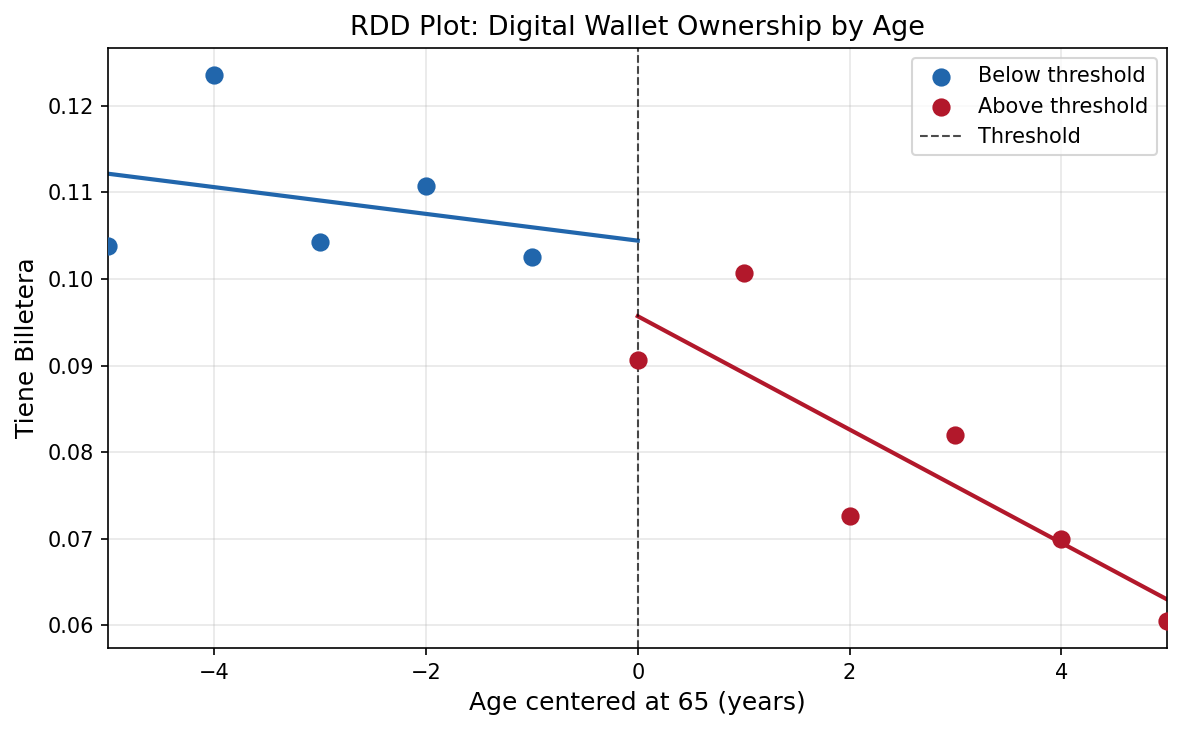
\includegraphics[width=0.9\textwidth]{figures/figure_1_rdplot.png}
\caption{RDD Plot: Digital Wallet Ownership by Age. Binned scatter with local-linear fit on each side of the cutoff. The vertical line marks age 65. There is no visible discontinuity at the cutoff.}
\label{fig:rdplot}
\end{figure}

\begin{figure}[H]
\centering
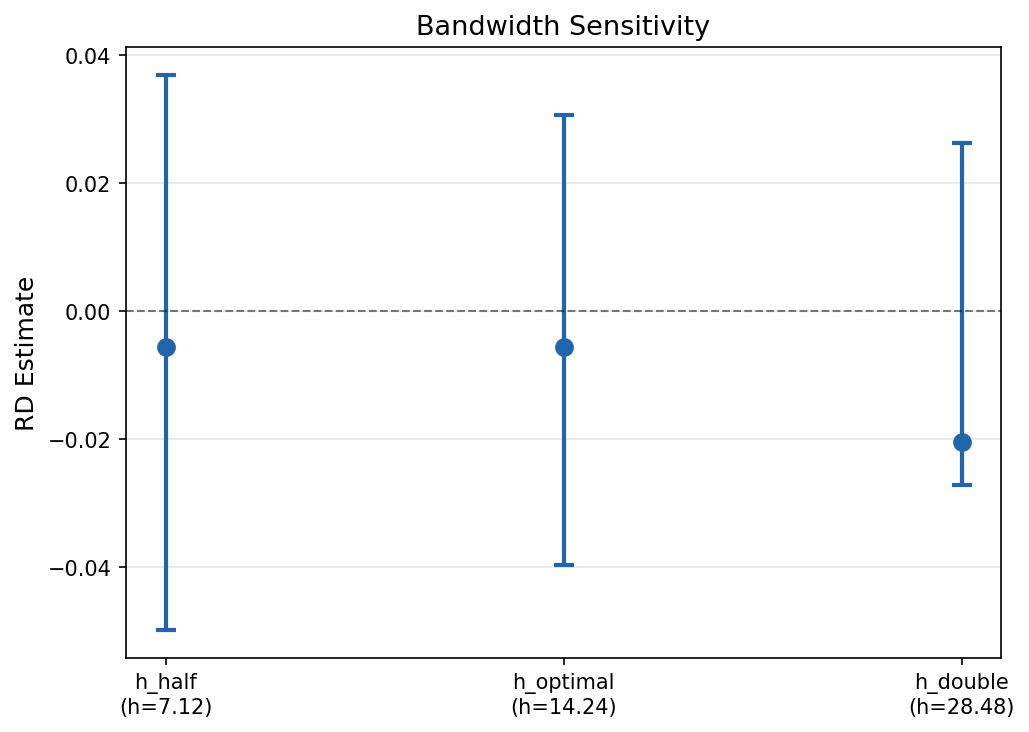
\includegraphics[width=0.9\textwidth]{figures/figure_2_bandwidth_sensitivity.png}
\caption{Bandwidth Sensitivity. Point estimates and 95\% confidence intervals for the primary outcome (\texttt{TIENE\_BILLETERA}) across bandwidth choices ranging from $h^*/2$ to $2 h^*$. The estimates are stable and confidence intervals consistently cover zero.}
\label{fig:bw_sensitivity}
\end{figure}

\begin{figure}[H]
\centering
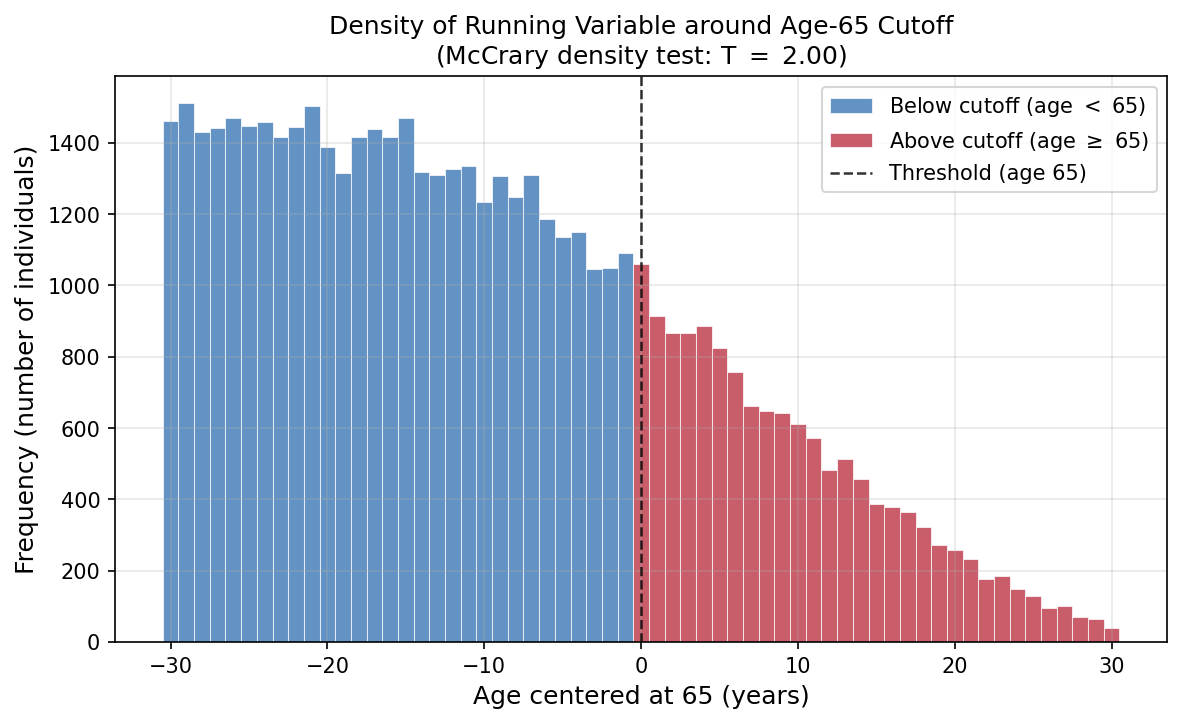
\includegraphics[width=0.9\textwidth]{figures/figure_mccrary_density.png}
\caption{Density of the Running Variable around the Age-65 Cutoff. The histogram displays the empirical density of age in the sample. While integer-age mass points are visible (a feature of self-reported age in years), there is no evidence of bunching specifically at age 65.}
\label{fig:mccrary}
\end{figure}


% =================================================================
% References
% =================================================================
\clearpage

\begin{thebibliography}{99}

\bibitem[Aizenman et~al.(2022)]{aizenman2022}
Aizenman, J., Jinjarak, Y., and Park, D. (2022).
Cash-Transfer Eligibility Thresholds and Digital Savings: Evidence from Latin America.
\textit{Journal of Development Economics}, 158:102934.

\bibitem[Ardington et~al.(2016)]{ardington2016}
Ardington, C., Case, A., and Hosegood, V. (2016).
Labor Supply Responses to Large Social Transfers: Longitudinal Evidence from South Africa.
\textit{American Economic Journal: Applied Economics}, 8(1):22--48.

\bibitem[Bachas et~al.(2018)]{bachas2018}
Bachas, P., Gertler, P., Higgins, S., and Seira, E. (2018).
Digital Financial Services Go a Long Way: Transaction Costs and Financial Inclusion.
\textit{AEA Papers and Proceedings}, 108:444--448.

\bibitem[Banerjee et~al.(2020)]{banerjee2020}
Banerjee, A., Niehaus, P., and Suri, T. (2020).
Universal Basic Income in the Developing World.
\textit{Annual Review of Economics}, 11:959--983.

\bibitem[Battistin et~al.(2009)]{battistin2009}
Battistin, E., Brugiavini, A., Rettore, E., and Weber, G. (2009).
The Retirement Consumption Puzzle: Evidence from a Regression Discontinuity Approach.
\textit{American Economic Review}, 99(5):2209--2226.

\bibitem[BCRP(2024)]{bcrp2024report}
Banco Central de Reserva del Per\'u (2024).
\textit{Reporte de Estabilidad Financiera, Noviembre 2024}.
Lima: BCRP.

\bibitem[Bruhn and Love(2014)]{bruhn2014}
Bruhn, M. and Love, I. (2014).
The Real Impact of Improved Access to Finance: Evidence from Mexico.
\textit{Journal of Finance}, 69(3):1347--1376.

\bibitem[Calonico et~al.(2014)]{calonico2014}
Calonico, S., Cattaneo, M.~D., and Titiunik, R. (2014).
Robust Nonparametric Confidence Intervals for Regression-Discontinuity Designs.
\textit{Econometrica}, 82(6):2295--2326.

\bibitem[Calonico et~al.(2019)]{calonico2019}
Calonico, S., Cattaneo, M.~D., Farrell, M.~H., and Titiunik, R. (2019).
Regression Discontinuity Designs Using Covariates.
\textit{Review of Economics and Statistics}, 101(3):442--451.

\bibitem[Card et~al.(2008)]{card2008}
Card, D., Dobkin, C., and Maestas, N. (2008).
The Impact of Nearly Universal Insurance Coverage on Health Care Utilization: Evidence from Medicare.
\textit{American Economic Review}, 98(5):2242--2258.

\bibitem[Cattaneo et~al.(2018)]{cattaneo2018}
Cattaneo, M.~D., Jansson, M., and Ma, X. (2018).
Manipulation Testing Based on Density Discontinuity.
\textit{Stata Journal}, 18(1):234--261.

\bibitem[Galiani et~al.(2020)]{galiani2020}
Galiani, S., Gertler, P., Bando, R., and Higgins, S. (2020).
Effect of the Digitization of Cash Transfers on Saving Behavior in Argentina.
\textit{World Bank Economic Review}, 34(Supplement):S57--S69.

\bibitem[Jack and Suri(2014)]{jack2014}
Jack, W. and Suri, T. (2014).
Risk Sharing and Transactions Costs: Evidence from Kenya's Mobile Money Revolution.
\textit{American Economic Review}, 104(1):183--223.

\bibitem[Muralidharan et~al.(2016)]{muralidharan2016}
Muralidharan, K., Niehaus, P., and Sukhtankar, S. (2016).
Building State Capacity: Evidence from Biometric Smartcards in India.
\textit{American Economic Review}, 106(10):2895--2929.

\bibitem[Suri(2017)]{suri2017}
Suri, T. (2017).
Mobile Money.
\textit{Annual Review of Economics}, 9:497--520.

\end{thebibliography}

\end{document}
